\documentclass[../../lecture_notes.tex]{subfiles}

\begin{document}

Memory management within a program is broken into two main categories:
\begin{enumerate} [itemsep=0mm]
	\item Stack Management
	\item Heap Management
\end{enumerate}

\subsubsection*{Stack Management}
Each function has an activation record called a frame that records the instance of the call.\\
Each frame shares the code, but the values are different.\\
A frame includes:
	\begin{itemize} [itemsep=0mm]
		\item return address
		\item arguments
		\item local variables
		\item temporary instances
	\end{itemize}

\noindent Frames developed in a few stages:
\begin{enumerate} [itemsep=0mm]
	\item FORTRAN (1958)\\
		Frames were static rather than dynamic; thus FORTAN had no stack or recursion
	\item C (1972) \\
		Frames statically defined frame layout, but the instantiation is left to runtime.\\
		This allows recursion!\\
		This does not allow for a heap, or global variables.
		\begin{lstlisting} [language=C]
		int f(int n) {
		  ... 
		  char[n] a; 
		  ...
		} // NOT ALLOWED
		\end{lstlisting}
	\item Algol (1960)\\
		Frames are stored in a stack which can grow as the program runs.\\
		Data is accessed by two pointers (\%rbp and \%rsp) to the base and top of the stack, respectively.
		\begin{lstlisting} [language=C++]
		int f(int n) {
		  ... 
		  char[n] a; 
		  ...
		} // OKAY
		\end{lstlisting}
		We can thus introduce the idea of \textbf{\underline{nested functions}}\\
		\begin{lstlisting} [language=C]
		int f(void) {
		  int x;
		  int g(void) {
		    int y;
		    ...
		    return x + y;
		  }
		  g();
		}
		f();
		\end{lstlisting}
	
		\begin{figure}[H]
			\centering
			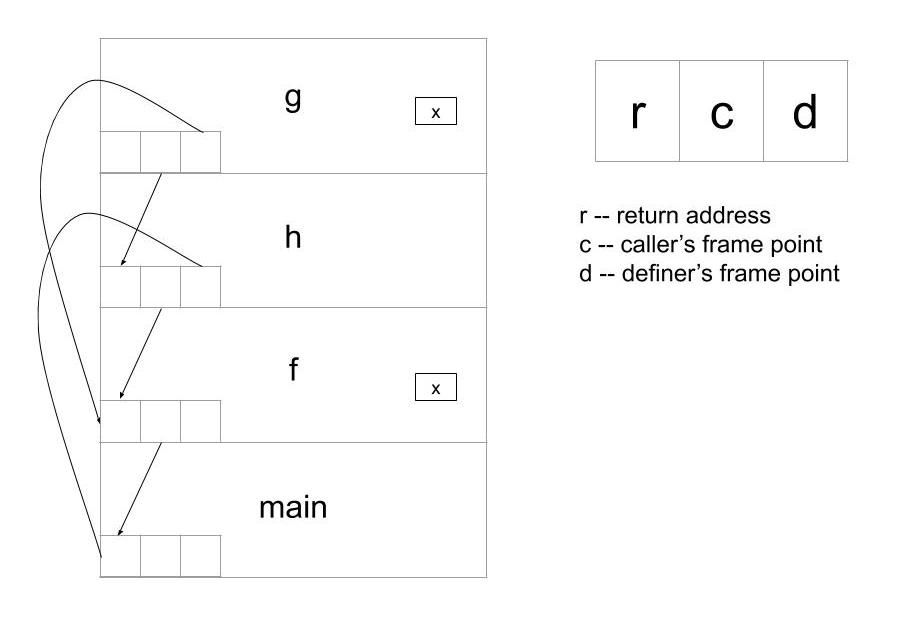
\includegraphics[width=\textwidth]{frames}
			\caption{A model nested function call}
			\label{fig:test}
		\end{figure}

		We store two linked lists of addresses.
		\begin{enumerate} [itemsep=0mm]
			\item \textbf{\underline{The Static Chain}}\\
				This forms the connection of definer frames.\\
				The depth is the nest level.\\
				This tends to be pretty short.
			\item \textbf{\underline{The Dynamic Chain}}\\
				This forms the connection of caller frames.\\
				The depth is the call level.\\
				This can be relatively long.
		\end{enumerate}

		To make this work, functions are represented by a pair of pointers
			\begin{enumerate} [itemsep=0mm]
				\item a pointer to the code (ip)
				\item a pointer to the defining frame (op)
			\end{enumerate}

		A function is thus an (ip, op) pair.\\
		These pointers are called FAT, since they hold two words as opposed to thin C pointers.\\
		This is how continuations work!

	\item ML
	A nesting function can return whilst the nested is still valid (currying).
		\begin{lstlisting} [language=ML]
	(fun x -> fun y -> x + y) 3;;
	-: 'a -> 'a = <fun>
	(* this returns a function that remembers the 3! *)
		\end{lstlisting}

	\begin{figure}[H]
		\centering
		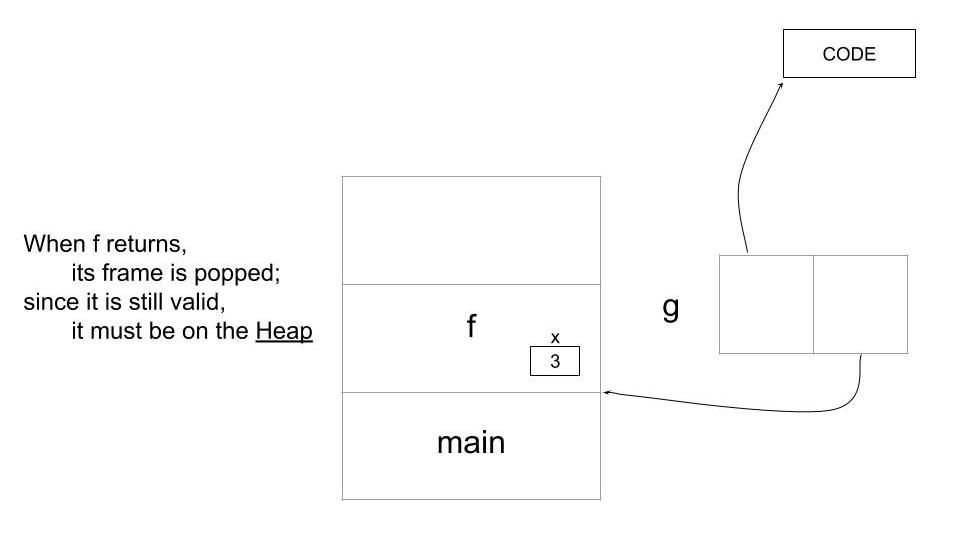
\includegraphics[width=\textwidth]{curry_frames}
		\caption{A currying frame}
		\label{fig:test}
	\end{figure}

\noindent The stack can be expanded or contracted with a single pointer addition instruction.\\
Thus heap management is far more expensive, so function calls are thus not as efficient.
\end{enumerate}

\subsubsection*{Heap Management}

\begin{figure}[H]
	\centering
	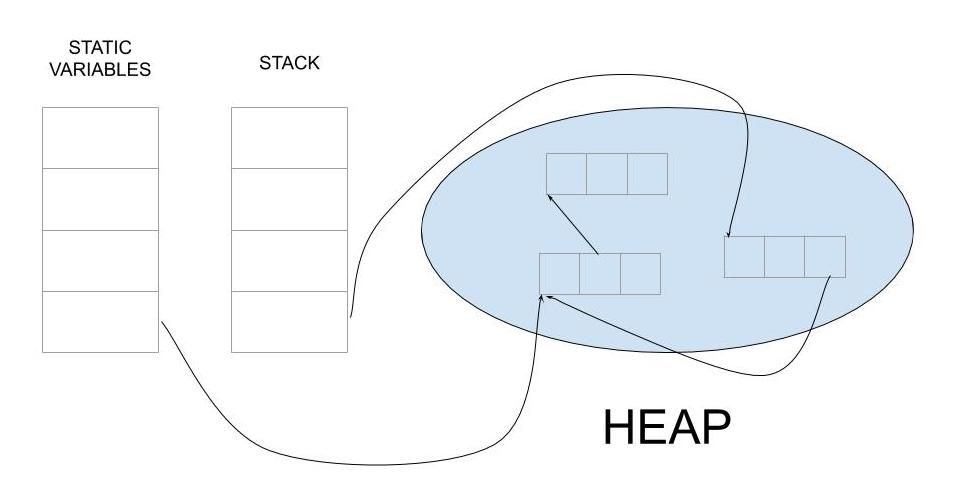
\includegraphics[width=\textwidth]{heap}
	\caption{}
	\label{fig:test}
\end{figure}

How do we arrange to free unused storage?\\
The simplest approach: explicit free operation\\
	\indent Problems:
	\begin{itemize} [itemsep=0mm]
		\item It is a hassle for the programmers.
		\item A programmer may forget to free. (memory leak!)
		\item A programmer may preemptively free. (dangling pointer → undefined access!)
	\end{itemize}

\noindent We can prevent this with \textbf{{garbage collection}}\\
	\indent $\equiv$ there is no ‘free’ — the underlying memory management system handles it.\\
	\indent Problems:
		\begin{itemize} [itemsep=0mm]
			\item How do we kept track of pointers into the heap (roots)?\\
				A static table is kept with a frame template and indirect pointers to the heap.
			\item How do we free indirect pointers to the heap?\\
				\textbf{\underline{mark \& sweep}}; 
					recursively mark all reachable elements, then free all unmarked.
			\item How does the heap managed keep track of used/unused space?\\
				We keep a free list in unused block 1 for fast allocation
		\end{itemize}

\begin{figure}[H]
	\centering
	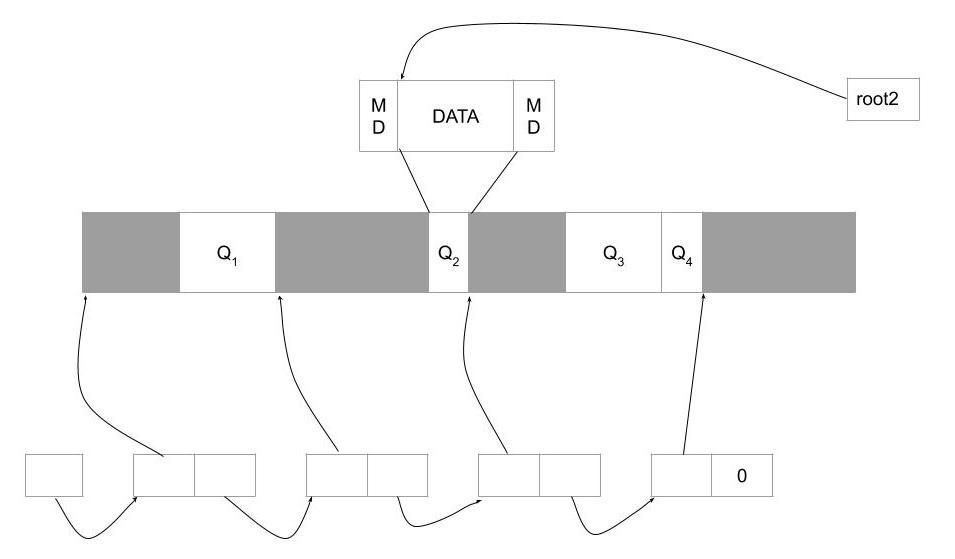
\includegraphics[width=\textwidth]{free_list}
	\caption{A model of a free list}
	\label{fig:test}
\end{figure}


\noindent The heap can become very large as the program’s data gets very large.\\
This can lead to delays, as memory allocation can take up to linear time.\\
Additionally, blocks near the beginning of the heap will tend to be more fragmented.\\
\indent If they fragment too much, they chew up CPU time as runts.\\
Thus we use a \textbf{\underline{roving pointer/next-fit list}}\\
	\indent $\equiv$ leave the free pointer at the location of the last successful allocation\\
\\
We must be sure to make a distinction between using a free/del operator \& a garbage collector.\\
If we are using free/del, keeping track of roots is delegated to the program.\\
The program is then responsible for not misusing the primitive (arbitrary free, double free, etc.).\\
This can be more efficient if the program is well written, BUT it is less reliable, since:
	\begin{itemize} [itemsep=0mm]
		\item Dangling Pointers (usage of freed storage)
		\item Memory Leaks (allocated and never freed memory)
		\item Imposter Pointers (free (void *) 2323; — luckily 2323 is not an address on SEASNet)
	\end{itemize}
The garbage collector is by far the most common choice in modern languages.\\
Thus garbage collectors avoid the above problems; how?
\begin{itemize} [itemsep=0mm]
	\item Storage is not reclaimed if it is reachable from roots.
	\item We want the GC to be as accurate as possible in determining which storage is reachable\\
	        BUT reclaiming immediately can be expensive, so we sometimes wait.
	\item Languages do not allow forging of pointers (in at least Java and OCaml)
\end{itemize} \smallskip

\noindent Mark and Sweep is generally a pretty good algorithm, but it makes malloc O(object count).\\
How can we speed it up?
\begin{enumerate} [itemsep=0mm]
	\item Mark and Sweep in a separate thread? NO — the locks will almost always be a bottleneck.
	\item Combine GC with C/C++? \\
		Our reflex is to say no, since
		\begin{enumerate} [itemsep=0mm] 
			\item C lets us theoretically access any address.
			\item The compiler doesn’t share roots or object layout with the program
		\end{enumerate}
\end{enumerate}

\noindent BUT it is possible with \textbf{\underline{conservative garbage collection}}.\\
\indent The garbage collector doesn’t know which data is a pointer, but it does have memory bounds.\\
\indent The objects that the heap manager knows about are:
	\begin{itemize} [itemsep=0mm]
		\item in registers (16 in x86-64)
		\item on the stack (\%rsp in x86-64)
		\item in static variables (*.o are static files)
	\end{itemize}
\indent We search in these locations and assume any pointers within range are valid

This can lead to issues:
	\begin{lstlisting} [language=C]
	char msg[] = "\300\147...";
	long long int gates_balance = 347140743208473;
	// might happen to be a pointer to the heap.
	malloc(1); // returned (char *)347140743208473 a while ago.  
	// The conservative GC will think that 1-byte object is still in use.
	\end{lstlisting}

\noindent BUT if we are careful, wrong-assumptions should be rare:\\
\indent We place our heap is in obscure locations, with addresses not likely to look like actual numbers.\\
If the wrong assumptions are rare, then we won’t have a lot of leaks.\\
\\
Who actually does the garbage collection?\\
\indent Typically garbage collection is done in user-mode code without much formal help.\\
This is done for performance reasons.\\
\\
The heap manager knows where objects are but does not show the OS.\\
For instance, one could find the source code for malloc() and free() written in C.\\
\indent (Mostly, except malloc could request a huge chunk of RAM)\\
This is a reasonably popular option and is used in the C++ gcc code and C emacs code.\\
The idea of this is that we never need to call free!
\begin{lstlisting}
		#define free(p) ((void*) p)
\end{lstlisting}

\noindent There are two major garbage collection methods:
	\begin{enumerate} [itemsep=0mm]
	\item \textbf{\underline{Generation-Based Copying Collector (Java)}}

		\begin{figure}[H]
			\centering
			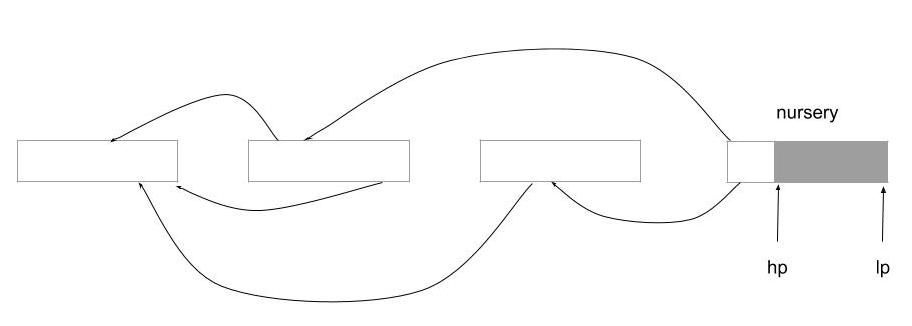
\includegraphics[width=\textwidth]{generational_heap}
			\label{fig:test}
		\end{figure}

		Older objects appear farther to the left; new allocations are taken from the nursery.\\
		Objects tend to point to older objects that rarely mutate, so garbage is in newer generations.\\
		In actuality, there is some overlap, since there are exceptions for backward pointers
		We thus only need to garbage collect the nursery, and the roots to a degree.\\
		The generation-based keyword refers to the the separately collected generations.\\

		\begin{figure}[H]
			\centering
			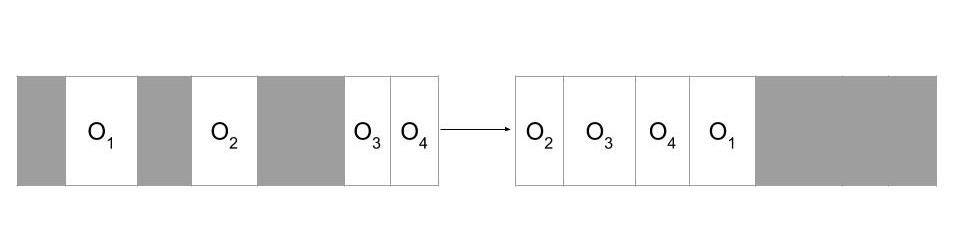
\includegraphics[width=\textwidth]{nursery_pack}
			\caption{Removing fragmentation from the nursery}
			\label{fig:test}
		\end{figure}

		The copying keyword comes from the merging to remove fragmentation.\\
		Upsides:
			\begin{enumerate} [itemsep=0mm]
				\item Runtime is O(bytes used).
				\item We need not access free areas.\\
					This might seem small, but avoiding a free list means 
						we don’t have to fill the L1 \& L2 cache.\\
					This is huge if the objects are small.
			\end{enumerate}
		Downsides:
			\begin{enumerate} [itemsep=0mm]
				\item We have to do a LOT of copying.
				\item We may need to free data not directly controlled by the GC.\\
				        We need to change any pointer referring to these objects.\\
				        We call Object.finalize() to collect garbage from a given object.\\
					This is a method that by default does nothing, and is for cleanup.\\
					mark and sweep can solve the finalize() issue.\\
					Upon sweep, unmarked objects have finalize() called.\\
				\end{enumerate} 
		Since this collector doesn’t sweep, Java has to blend the two approaches:\\
		Java does generation-based garbage collection for standard objects.\\
		It does mark and sweep for objects with a user-defined finalize() method.\\
\\
		ISSUE — Multithreading.\\
		The naive multithreaded garbage collector requires synchronization, and thus is slow.\\
		Java avoids a global lock by giving each nursery its own lock.\\
		Typically, threads share only old objects, so in practice this works well.\\
		In the worst case, this reduces to the global lock case.\\
\\
		ISSUE — Real-Time.\\
		In this case, we don’t care particularly about the speed of ‘new’, but predictability.\\
		Thus we do an incremental garbage collection with some marking or sweeping each call.\\
		This can be tricky, but is often used in Java applications.\\


	\item \textbf{\underline{Reference-Counting Garbage Collector (C-Python)}}\\
		Each object keeps track of the number of references to it.

		\begin{figure}[H]
			\centering
			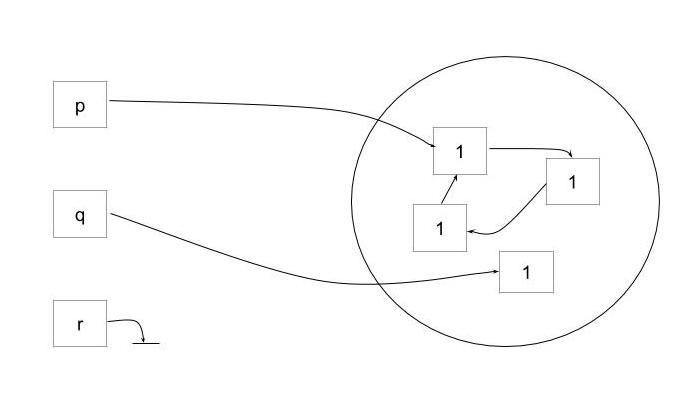
\includegraphics[width=0.6\textwidth]{Python_heap}
			\caption{A model nested function call}
			\label{fig:test}
		\end{figure}


		Positives:
			\begin{enumerate} [itemsep=0mm]
				\item quick garbage discovery/reclamation
			\end{enumerate}
		Negatives:
			\begin{enumerate} [itemsep=0mm]
				\item cyclic object patterns are not reclaimed
				\item Lost references
			\end{enumerate}

		Not having cycles isn’t inherently terrible, but people laughed off Python’s method.\\
		This is because they either needed avoid cycles or remember to break them.\\
		Nowadays, Python integrates an extra phase of mark \& sweep.\\
		The timing of the mark and sweep is dependent on multiple heuristically tuned parameters.\\
		Therefore, we need to optimize these when building a large application.\\
\\
		A trick that sometimes works and sometimes fails miserably is called \textbf{\underline{object polling}}.\\
		Say we know we are going to allocate a bunch of ‘struct cons’ objects. We then do\\
		\begin{lstlisting} [language=C]
	struct cons { struct cons * car; struct cons *cdr; }; 
	// We thus allocate en masse and keep our own free list
	struct cons *free_conses;
	struct cons *next_cons(void) {
	  if (free_conses) {
	    struct cons * r = free_conses;
	    free_conses = r->car;
	    return r;
	  }
	  return malloc(sizeof(struct cons)); // expensive
	}
	void free_cons(struct cons *p) {
	  p->car = free_conses;
	  free_conses = p;
	}
		\end{lstlisting}
    This works with mark and sweep, is but terrible for generation, since it copies the free list.
\end{enumerate}
\end{document}